\documentclass[../report.tex]{subfiles}
\begin{document}   

\subsection{Introduction}

With over 100 million monthly listeners\cite{musicoomph} and a steadily increasing user base, there is no doubt that podcasts are a greatly enriching source of information and entertainment for a large variety of individuals.

Although they are highly valuable, it can be difficult to find podcasts that are of interest to a particular user amidst the 1 million\cite{musicoomph} that are already available.
Thus, podcast streaming services (such as UltraCast) have been created, to provide a centralised place for exploring and discovering new podcasts that are valuable to the listener.

However, all of the web based podcast streaming services available lack many important features, and their interfaces leave much to be desired. For example, there is no streaming service that allows the user to bookmark certain parts of a podcast, nor take notes at certain timestamps. It is even difficult to find a service that allows the listener to change the playback speed of the podcast.

UltraCast combines all of the most important features together into a single package with a web-based podcast streaming service.

UltraCast differentiates itself from competitors by allowing users to:
\begin{itemize}
    \item Follow friends to see what they have been listening to
    \item Create \textit{Streams} of podcasts to find interesting podcasts
    \item Create bookmarks inside podcast episodes
    \item Monitor episode and podcast play metrics
\end{itemize}

\subsection{Project Requirements}
The minimun project requirements from the specifications are:
\begin{itemize}
    \item Listeners must be able to search for podcasts that interest them by keywords, resulting in a list of matching podcast titles, where the total number of subscriptions on the UltraCast platform (function described later) for each podcast is shown next to the title
    \item Listeners must be able to select a podcast show from returned search results to view its full details, including its title, description, any author details that exist, as well as a list of episodes for the show 
    \item Listeners must be able to play a selected episode within a podcast show, and once that episode starts being played, the listener must be able to also clearly see this episode marked as "Played" 
    \item Listeners must be able to subscribe or unsubscribe from a podcast show         Listeners must be able to see the latest episode available for each show that they subscribed to in a "Podcast Subscription Preview" panel
    \item Listeners must be notified by the platform when a new episode for a show  they are subscribed appears
    \item Listeners must be able to see a history of the podcast episodes that they have played, sorted in order from most recently played to least recently played
    \item UltraCast must be able to recommend new podcast shows to a listener based on at least information about the podcast shows they are subscribed to, podcast episodes they have recently played, and their past podcast searches
\end{itemize}
%
The following additional requirements have also been implemented:
\begin{itemize}
    \item Listeners should be able to follow their \textit{friends} and view the podcasts that their \textit{friends} have recently listened to
    \item Listeners should be able to create \textit{Streams} based off search queries that they can use to find interesting podcasts
    \item Listeners should be able to add bookmarks with a name and description to podcast episodes as they listen to them
    \item Content creators should be able to create and upload podcasts and podcast episodes
    \item Content creators should be able to monitor analytics of their uploaded podcasts related to their listeners
\end{itemize}

\newpage

\subsection{System Architecture}

The highlevel system architecture can be seen in Figure \ref{fig:system_architecture}.
It can be seen that our end users will be podcast listeners and content creators who
connect to the presentation layer which is powered by a ReactJS application. ReactJS was selected as
the framework for the frontend application due to .... TODO justification of React\\

Flask, a micro-framework, \cite{flask} was used for the web-server, due ease of use which allowed
for rapid development. The React application communicates with Flask web-server through a GraphQL API: 
a scalable alternative to the popular REST API\cite{graphql}. The Flask web-server also contains a
recommendation service which drives recommendation functionality described in TODO. The Flask
web-server uploads static files (episode audio and podcast covers) to a static file storage server while
the urls for these static files along with all other data is stored in MongoDB. MongoDB, a NoSQL database, 
was selected to store metadata due to its scalability \cite{MongoDB2020}.

\begin{figure}[ht] 
    \centering
    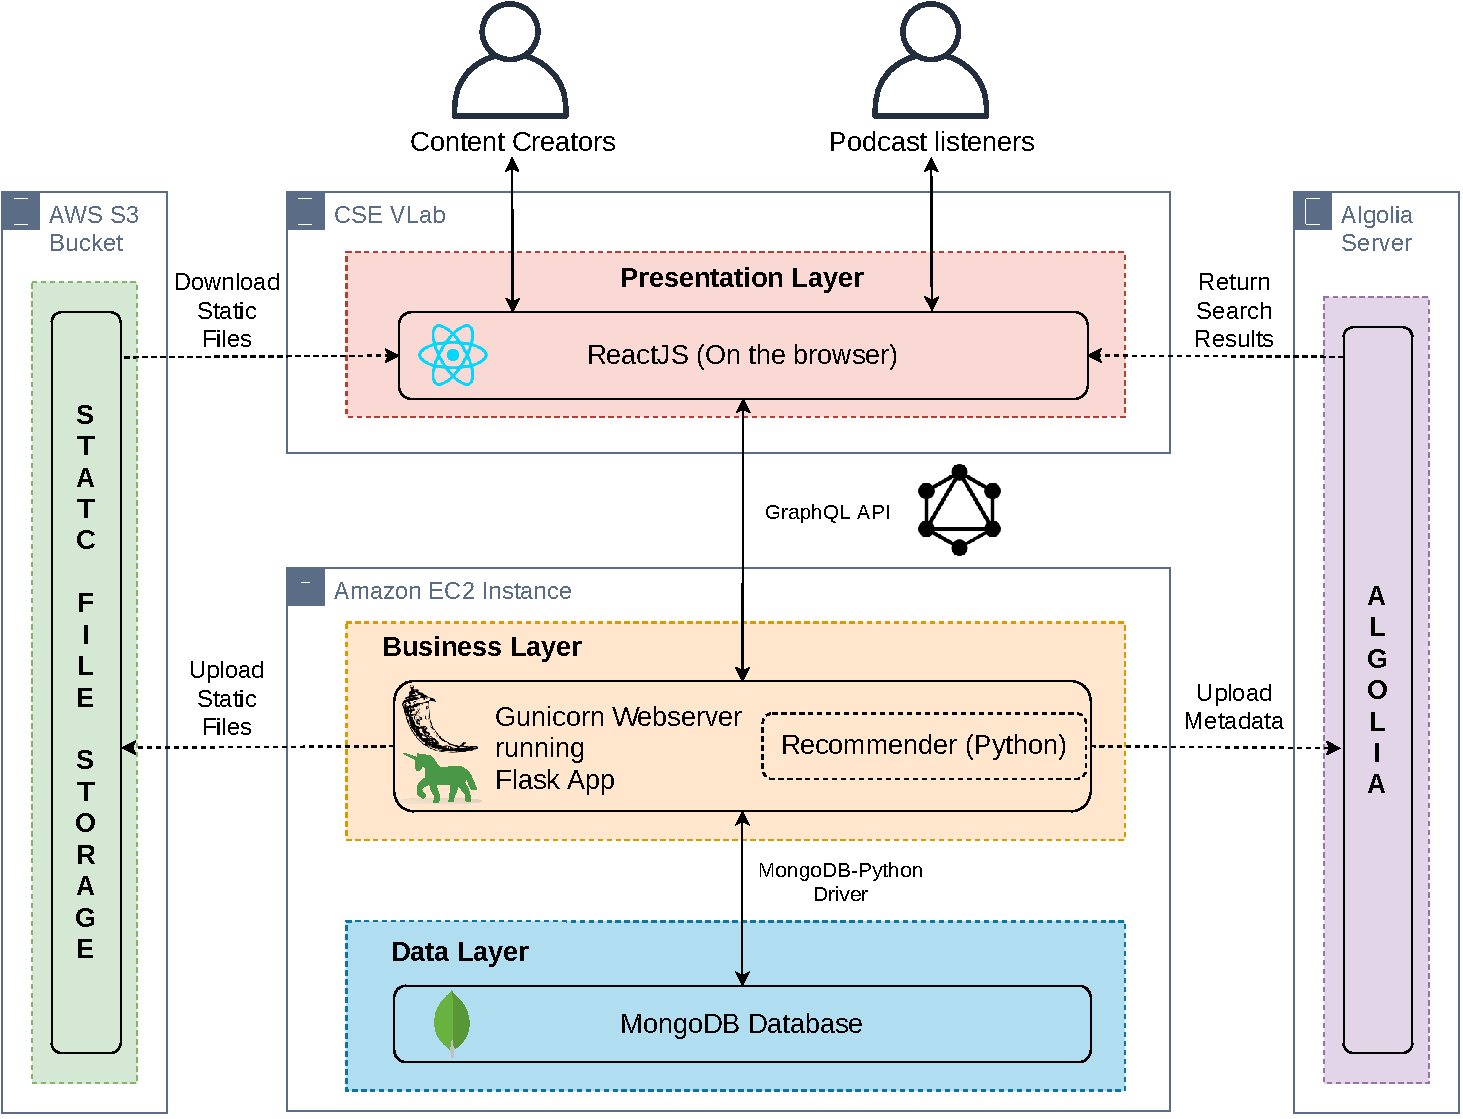
\includegraphics[width=16cm]{resources/SystemArchitecture}
    \caption{UltraCast System Architecture}
    \label{fig:system_architecture} 
\end{figure}

A static file storage server (AWS S3 Bucket) was used instead of MongoDB due to the lower costs 
and increased performance associated with storing larger files, particularly audio files TODO-cite.
MongoDB was not supported by Debian 6 (the Linux environment on the VLab machine), so a remote server
(AWS EC2 instance) was used to host MongoDB. To improve query performance, the entire business layer
was migrated to the remote server. (TODO - should probs cite why query performance improved)


\end{document}
